% Provenance (never printed): old terminale S material on the Earth's internal
% heat (geothermal gradient and heat flow, radioactive heat production,
% conduction and convection, mantle convection, geothermal energy). Owner
% (Sync 0/1): heat flow, radiogenic heat production, secular cooling, thermal
% and mantle convection (recall the convection cell of Book 1 g8 first),
% geothermal energy. Geotherm and geothermal gradient are g11.03's; radioactivity,
% half-life, decay law and thermal conductivity are physics' (thermal
% conductivity used as "the rock's thermal conductivity k", never defined);
% hotspot track and plume g11.04's. Figures: figdata/grade-12/internal_heat.py.
\chapter{La chaleur interne de la Terre}\label{ch:g12:internal-heat}

Entre 1987 et 1995, près du village de Windischeschenbach, en Bavière, des
géologues ont foré un trou de \qty{9101}{m} de profondeur dans la \omterm{def:g12:continental-crust:continental-crust}{croûte
continentale}. Au fond, la roche était à environ \qty{265}{\celsius}~: trop
chaude pour forer plus loin.
% ledger: gfz:ktb, gfz:ktb30

Passer d'environ \qty{10}{\celsius} en surface à \qty{265}{\celsius} à
\qty{9.1}{km}, c'est une hausse d'environ \qty{28}{\celsius} par
kilomètre, une valeur typique. Partout sur Terre, la température augmente
vers le bas~: la chaleur sort donc de la Terre en permanence. Ce chapitre
mesure ce flux, cherche d'où vient la chaleur, et montre comment elle se
déplace.
% values: ktb_gradient 28.0 (internal_heat.py, surface temperature taken as 10 degC); ledger: gfz:ktb (gradient about 28 K/km)

\begin{recall}
Le \omterm{def:g11:lithosphere-asthenosphere:geotherm}{géotherme} est la courbe de la température en fonction de la profondeur
sous un lieu, et le \omterm{def:g11:lithosphere-asthenosphere:geotherm}{gradient géothermique} la hausse de température par
kilomètre~; les forages mesurent 25 à \qty{30}{\celsius} par kilomètre
près de la surface (\cref{ch:g11:lithosphere-asthenosphere}). Certains
atomes sont radioactifs~: ils se désintègrent au hasard, leur nombre
diminuant de moitié à chaque demi-vie, et chaque désintégration libère de
l'énergie, qui finit en chaleur (les livres de physique). Une cellule de
convection est une boucle de fluide chauffé par le bas, qui monte, s'étale,
se refroidit et redescend (livre~1, année~8). À un point chaud, une plaque
se déplace au-dessus d'un panache de manteau chaud
(\cref{ch:g11:plate-motions}).
\end{recall}
% ledger: usgs:gradient-29 (Book 1 row)

\section{Gradient et flux géothermique}

\begin{definition}[Flux géothermique]\label{def:g12:internal-heat:heat-flow}
Le \emph{flux géothermique}\index{flux geothermique@flux géothermique} (ou
flux de chaleur) en un lieu est la puissance qui sort de l'intérieur de la
Terre à travers chaque mètre carré de sa surface en ce lieu. On le mesure
en milliwatts par mètre carré (\unit{mW/m^2}).
\end{definition}
% ledger: b2dd10:continents

La chaleur va du chaud vers le froid, et plus le gradient de température
est fort, plus elle s'écoule vite. La quantité qui passe dépend aussi de la
roche~: chaque roche a une conductivité thermique $k$, en watts par mètre
et par kelvin, que définissent les livres de physique.

\begin{proposition}[Flux géothermique et gradient]\label{prop:g12:internal-heat:fourier}
À travers une roche de conductivité thermique $k$ dans laquelle la
température augmente avec la profondeur selon un gradient $G$ (en kelvins
par mètre), le \omterm{def:g12:internal-heat:heat-flow}{flux géothermique} dirigé vers la surface vaut
\[
  q = k\,G .
\]
\end{proposition}

Cette loi de la conduction, due à Fourier, est admise ici~; les livres de
physique la démontrent sous une forme générale.

\begin{method}[Un flux géothermique à partir d'un forage]\label{met:g12:internal-heat:borehole}
\begin{enumerate}
  \item Mesurer la température à plusieurs profondeurs d'un forage, une
        fois que le trou a eu le temps de revenir à la température de la
        roche.
  \item Tracer la température en fonction de la profondeur et prendre la
        pente~: c'est le gradient $G$, converti en kelvins par mètre.
  \item Mesurer la conductivité $k$ de la roche sur des carottes, au
        laboratoire.
  \item Multiplier~: $q = kG$, en \unit{W/m^2}, puis convertir en
        \unit{mW/m^2}.
\end{enumerate}
\end{method}

\begin{example}[Un forage dans un granite]\label{ex:g12:internal-heat:borehole}
Un forage dans un granite de conductivité \qty{2.72}{W/(m.K)} mesure un
gradient de \qty{29}{\celsius} par kilomètre, soit \qty{0.029}{K/m}.
Alors $q = 2.72 \times 0.029 \approx \qty{0.079}{W/m^2}$, environ
\qty{79}{mW/m^2}.
\end{example}
% ledger: roy:conductivity (granitic layer 6.5 mcal/(cm s degC) = 2.72 W/m/K), usgs:gradient-29 (Book 1 row)
% values: borehole_q_mW 78.9 (internal_heat.py)

Plus de 38\,000 mesures de ce type ont été réunies en une carte de la
Terre entière. Les continents perdent en moyenne \qty{70.9}{mW/m^2}, les
fonds océaniques \qty{105.4}{mW/m^2}~; sur toute la surface,
\qty{91.6}{mW/m^2}. Multiplié par la surface de la Terre,
\qty{5.101e14}{m^2}, le total vaut
\[
  0.0916 \times \num{5.101e14} \approx \qty{4.67e13}{W} = \qty{46.7}{TW},
\]
environ 47 térawatts, à 2 près.
% ledger: b2dd10:continents, b2dd10:half-space (47 +- 2 TW, 38,347 measurements)

Les fonds océaniques perdent le plus là où ils sont les plus jeunes. La
\omterm{def:g11:lithosphere-asthenosphere:lithosphere}{lithosphère} nouvelle quitte la dorsale chaude, et se refroidit en
s'éloignant~; son \omterm{def:g12:internal-heat:heat-flow}{flux géothermique} diminue comme l'inverse de la racine
carrée de son âge.

\begin{omfigure}
\begin{tikzpicture}
\begin{axis}[omrecord, width=0.72\linewidth, height=5.6cm, xmin=0, xmax=180, ymin=0, ymax=400,
  xlabel={âge des fonds océaniques (millions d'années)}, ylabel={flux géothermique (\unit{mW/m^2})},
  xtick={0,30,...,180}, ytick={0,100,...,400}]
% computed in figdata/grade-12/internal_heat.py; ledger: b2dd10:half-space, b2dd10:continents
\addplot[omDef, line width=1.1pt, restrict x to domain=0:66.5] table[x=t_Myr, y=q] {figdata/out/grade-12-internal_heat-halfspace.dat};
\addplot[omDef, line width=1.1pt, densely dotted, restrict x to domain=66.5:180] table[x=t_Myr, y=q] {figdata/out/grade-12-internal_heat-halfspace.dat};
\addplot[omProp, line width=0.9pt, dashed, domain=0:180] {70.9};
\coordinate (lawlab) at (axis cs:14,250);
\coordinate (contlab) at (axis cs:100,80);
\end{axis}
\node[font=\scriptsize, text=omDef, anchor=west] at (lawlab) {$q = 490/\sqrt{t}$};
\node[font=\scriptsize, text=omProp, anchor=south west] at (contlab) {moyenne des continents, \qty{70.9}{mW/m^2}};
\end{tikzpicture}

{\small Le \omterm{def:g12:internal-heat:heat-flow}{flux géothermique} à travers les fonds océaniques en fonction de
leur âge, tel qu'il est calculé pour le refroidissement de la \omterm{def:g11:lithosphere-asthenosphere:lithosphere}{lithosphère}
($t$ en millions d'années)~; au-delà de 66.5 millions d'années (en
pointillés), on sait que la loi convient moins bien. Source~: Davies et
Davies (2010).}
\end{omfigure}
% values: q_1Myr 490, q_10Myr 155, q_66.5Myr 60.1, age_where_q_equals_cont_Myr 47.8 (internal_heat.py)

\section{D'où vient la chaleur~?}

La chaleur a deux sources. La première est la radioactivité.

\begin{definition}[Production de chaleur radiogénique]\label{def:g12:internal-heat:heat-production}
La \emph{production de chaleur radiogénique}\index{production de chaleur radiogenique@production de chaleur radiogénique}
d'une roche est la chaleur libérée en elle par la désintégration de ses
atomes radioactifs, par unité de volume et de temps, en microwatts par
mètre cube (\unit{\micro W/m^3}). Elle provient presque entièrement de
quatre isotopes~: l'uranium~238, l'uranium~235, le thorium~232 et le
potassium~40.
\end{definition}
% ledger: dye12:isotopes, earle:heat-sources, kamland11:geonu

Ces éléments sont concentrés dans les roches de la \omterm{def:g12:continental-crust:continental-crust}{croûte continentale}.
D'après 2188 analyses, la production de chaleur médiane du granite est de
\qty{2.43}{\micro W/m^3}, celle du basalte de \qty{0.21}{\micro W/m^3}, et
celle des roches ultramafiques du manteau de seulement
\qty{0.11}{\micro W/m^3}, environ vingt fois moins que le granite. Une
couche de granite de \qty{10}{km} d'épaisseur produit
$2.43 \times 10^{-6} \times \num{10000} \approx \qty{0.024}{W}$ sous chaque
mètre carré, soit \qty{24}{mW/m^2}~: le tiers du \omterm{def:g12:internal-heat:heat-flow}{flux géothermique} des
continents.
% ledger: b2vila:heat-production, b2dd10:continents
% values: granite_10km_mW 24.3, granite_over_ultramafic 21.9 (internal_heat.py)

Combien de chaleur la radioactivité produit-elle dans la Terre entière~?
KamLAND, un détecteur souterrain installé au Japon et contenant 1000 tonnes
de liquide, capte les géoneutrinos, les antineutrinos libérés par la
désintégration de l'uranium et du thorium à l'intérieur de la Terre~: il a
vu les premiers en 2005, puis, en 2135 jours d'enregistrement, environ 106
d'entre eux parmi 841 événements candidats. D'après ce comptage, joint à
celui d'un détecteur installé en Italie, l'uranium~238 et le thorium~232
libèrent ensemble environ 20 térawatts. Le potassium~40 échappe au
détecteur~; on sait qu'il ajoute environ \qty{4}{TW}, et l'uranium~235,
déduit de l'uranium~238, environ \qty{0.4}{TW}. La radioactivité fournit
donc environ \qty{24}{TW}, à peu près la moitié des \qty{47}{TW} que perd
la Terre.
% ledger: kamland11:geonu, dye12:isotopes, b2dd10:continents
% values: now_K40_TW 4.0, now_U235_TW 0.42, radiogenic_TW 24.4, share_radiogenic 0.523 (internal_heat.py)

\begin{definition}[Refroidissement séculaire]\label{def:g12:internal-heat:secular-cooling}
Le \emph{refroidissement séculaire}\index{refroidissement seculaire@refroidissement séculaire}
de la Terre est la lente perte de la chaleur qu'elle a emmagasinée depuis sa
formation, la chaleur primordiale~: c'est la part du \omterm{def:g12:internal-heat:heat-flow}{flux géothermique} que
la radioactivité ne remplace pas, et par laquelle le manteau et le noyau se
refroidissent au fil des âges.
\end{definition}
% ledger: kamland11:geonu, earle:heat-sources

\begin{omfigure}
\begin{tikzpicture}
\begin{axis}[omrecord, xbar stacked, bar width=14pt, width=0.66\linewidth, height=3.2cm, scale only axis,
  xmin=0, xmax=50, ymin=0.4, ymax=2.6, ytick={1,2}, yticklabels={{sources}, {pertes}},
  xlabel={puissance (\unit{TW})}, ymajorgrids=false, legend columns=2, legend cell align=left,
  legend style={font=\scriptsize, at={(0.5,-0.42)}, anchor=north, /tikz/every even column/.append style={column sep=6pt}}]
% computed in figdata/grade-12/internal_heat.py; ledger: kamland11:geonu, dye12:isotopes, b2dd10:continents
\addplot[fill=omThm!55, draw=omThm] table[x=uth, y=bar] {figdata/out/grade-12-internal_heat-budget.dat};
\addplot[fill=omThm!25, draw=omThm] table[x=kuf, y=bar] {figdata/out/grade-12-internal_heat-budget.dat};
\addplot[fill=omDef!35, draw=omDef] table[x=secular, y=bar] {figdata/out/grade-12-internal_heat-budget.dat};
\addplot[fill=black!25, draw=black!60] table[x=surface, y=bar] {figdata/out/grade-12-internal_heat-budget.dat};
\legend{{uranium 238 et thorium 232 (géoneutrinos)}, {potassium 40 et uranium 235}, {refroidissement séculaire (le reste)}, {flux géothermique en surface}}
\end{axis}
\end{tikzpicture}

{\small Le bilan thermique actuel de la Terre~: ce qui sort par la surface
(barre du haut) et ce qui l'alimente (barre du bas). Sources~: KamLAND
(2011)~; Davies et Davies (2010)~; Dye (2012).}
\end{omfigure}
% values: radiogenic_TW 24.4, secular_TW 22.3 (internal_heat.py)

La radioactivité était plus forte dans le passé. Chaque isotope se
désintègre~: il y en avait donc davantage autrefois~; une demi-vie plus
tôt, deux fois plus, et deux fois plus de chaleur. Remonter de $t$ années
multiplie la chaleur d'un isotope de demi-vie $T$ par $2^{t/T}$.

\begin{proposition}[La chaleur radiogénique dans le passé]\label{prop:g12:internal-heat:past}
Si un isotope de demi-vie $T$ libère aujourd'hui une puissance $H_0$, il
libérait
\[
  H(t) = H_0 \, 2^{t/T} = H_0\, e^{\lambda t}, \qquad \lambda = \frac{\ln 2}{T},
\]
il y a un temps $t$.
\end{proposition}

\begin{proof}
La puissance est proportionnelle au nombre $N$ d'atomes qui restent,
puisque chacun se désintègre avec la même probabilité par seconde. D'après
la loi de décroissance, $N$ est divisé par 2 à chaque demi-vie~:
$N_{\text{auj}} = N(t)\,2^{-t/T}$, donc $N(t) =
N_{\text{auj}}\,2^{t/T}$, d'où la puissance. Enfin, $2^{t/T} =
e^{(t/T)\ln 2} = e^{\lambda t}$.
\end{proof}

\begin{omfigure}
\begin{tikzpicture}
\begin{axis}[omrecord, width=0.72\linewidth, height=6cm, xmin=0, xmax=4.5, ymin=0, ymax=120,
  x dir=reverse, xlabel={temps avant l'actuel (milliards d'années)}, ylabel={chaleur radiogénique (\unit{TW})},
  xtick={0,0.5,...,4.5}, ytick={0,20,...,120}, x tick label style={/pgf/number format/.cd, fixed, precision=1},
  legend pos=north east, legend style={font=\scriptsize}, legend cell align=left]
% computed in figdata/grade-12/internal_heat.py; ledger: kamland11:geonu, dye12:isotopes, nndc:halflives
\addplot[black, line width=1.2pt] table[x=t_Ga, y=total] {figdata/out/grade-12-internal_heat-past.dat};
\addplot[omThm, line width=0.9pt] table[x=t_Ga, y=U235] {figdata/out/grade-12-internal_heat-past.dat};
\addplot[omProp, line width=0.9pt, densely dashed] table[x=t_Ga, y=K40] {figdata/out/grade-12-internal_heat-past.dat};
\addplot[omDef, line width=0.9pt] table[x=t_Ga, y=U238] {figdata/out/grade-12-internal_heat-past.dat};
\addplot[omMeth, line width=0.9pt, densely dotted] table[x=t_Ga, y=Th232] {figdata/out/grade-12-internal_heat-past.dat};
\legend{total, uranium 235, potassium 40, uranium 238, thorium 232}
\end{axis}
\end{tikzpicture}

{\small La chaleur libérée par les quatre isotopes radioactifs depuis la
formation de la Terre, calculée à partir des valeurs actuelles avec la loi
de décroissance. Demi-vies~: thorium~232, 14.0~milliards d'années~;
uranium~238, 4.468~; potassium~40, 1.248~; uranium~235, 0.704.}
\end{omfigure}
% values: total_4.5Ga_TW 115.9, ratio_total_4.5Ga 4.75, ratio_U235_4.5Ga 84.0, ratio_K40_4.5Ga 12.2, share_U235_K40_4.5Ga 0.72 (internal_heat.py)

Il y a quatre milliards et demi d'années, la radioactivité libérait environ
\qty{116}{TW}, presque cinq fois la valeur actuelle, et l'essentiel venait
de l'uranium~235 et du potassium~40, les deux isotopes à vie courte, qui
ont depuis presque disparu. La jeune Terre était bien plus chaude à
l'intérieur qu'aujourd'hui.
% ledger: earle:heat-sources (radiogenic heat now roughly 25 % of what it was)

\section{Conduction et convection}

La chaleur ne peut traverser un solide que par conduction, d'atome en atome,
et dans la roche c'est très lent. La chaleur traverse par conduction une
distance $L$ en un temps d'environ $L^2/\kappa$, où $\kappa$, la
diffusivité thermique de la roche, vaut environ \qty{1e-6}{m^2/s}. Pour les
\qty{2891}{km} du manteau,
\[
  \frac{(\num{2.891e6})^2}{\num{1e-6}} \approx \qty{8.4e18}{s} \approx
  \num{2.6e11} \text{ ans},
\]
soit quelque 260 milliards d'années, près de soixante fois l'âge de la
Terre. Si le manteau ne faisait que conduire la chaleur, la chaleur de ses
profondeurs y serait encore presque entièrement.
% ledger: england:kelvin (Book 3 row: kappa 1e-6 m2/s), data:prem (CMB at 2891 km)
% values: conduction_time_Gyr 264.9 (internal_heat.py)

Le manteau est solide, mais à l'échelle de millions d'années il flue, très
lentement, comme un fluide très visqueux~: l'\omterm{def:g11:lithosphere-asthenosphere:lithosphere}{asthénosphère} s'écoule
(\cref{ch:g11:lithosphere-asthenosphere}). Le manteau perd donc sa chaleur
comme l'air au-dessus d'un radiateur, en la transportant.

\begin{definition}[Convection thermique~; convection mantellique]\label{def:g12:internal-heat:convection}
La \emph{convection thermique}\index{convection thermique} est le transport
de chaleur par le mouvement de la matière elle-même~: la matière plus
chaude et plus légère monte, la matière plus froide et plus dense descend,
comme dans une cellule de convection. La \emph{convection
mantellique}\index{convection mantellique} est la convection thermique du
manteau solide de la Terre, qui flue à quelques centimètres par an et
transporte la chaleur de l'intérieur vers la surface.
\end{definition}
% ledger: earle:heat-sources (solid mantle flows at centimetres a year)

Les plaques sont la partie supérieure de cette convection. Aux dorsales, du
manteau chaud monte et s'ajoute aux plaques~; la \omterm{def:g11:lithosphere-asthenosphere:lithosphere}{lithosphère} se refroidit en
s'éloignant, devient dense, et s'enfonce sous son propre poids aux \omterm{def:g11:subduction-zones:subduction}{zones de
subduction}~: les \omterm{def:g11:subduction-zones:slab}{panneaux plongeants} sont la partie froide et descendante
de l'écoulement, et l'imagerie sismique les montre s'enfonçant
profondément dans le manteau. On pense que des panaches de roche chaude
montent sous les points chauds depuis les profondeurs du manteau,
peut-être depuis le voisinage immédiat du noyau.
% ledger: dye12:bse, earle:plume

\begin{omfigure}
\begin{tikzpicture}[x=1cm, y=1cm, font=\scriptsize]
  % mantle annulus sector
  \fill[omLithPeridotite!40] (0,0) ++(20:6.4) arc (20:160:6.4) -- ++(160:-3.2) arc (160:20:3.2) -- cycle;
  \fill[black!45] (0,0) ++(20:3.2) arc (20:160:3.2) -- (0,0) -- cycle;
  \node[white] at (0,1.6) {noyau};
  % lithosphere
  \fill[black!15, draw=black!50] (0,0) ++(20:6.4) arc (20:160:6.4) -- ++(160:-0.3) arc (160:20:6.1) -- cycle;
  % ridge (top) and two trenches
  \draw[omThm, line width=1pt, -{Stealth}] (0,5.9) -- (0,6.35);
  \node[anchor=south] at (0,6.45) {dorsale};
  \foreach \a/\lab in {48/fosse, 132/fosse} {
    \node[anchor=south] at (\a:6.5) {\lab};
  }
  % slabs (cold, blue) sinking from the trenches
  \draw[omDef, line width=3pt] (48:6.2) .. controls (52:5.2) and (60:4.4) .. (62:3.4);
  \draw[omDef, line width=3pt] (132:6.2) .. controls (128:5.2) and (120:4.4) .. (118:3.4);
  % plume (hot, red) rising
  \draw[omThm, line width=2.4pt] (155:3.25) .. controls (154:4.2) and (152:5.2) .. (151:6.05);
  \fill[omThm] (151:6.0) circle (0.18);
  \node[anchor=west, text=omThm] at (145:4.0) {panache~?};
  % convection arrows
  \draw[-{Stealth}, black!65, line width=0.8pt] (80:5.7) arc (80:58:5.7);
  \draw[-{Stealth}, black!65, line width=0.8pt] (100:5.7) arc (100:122:5.7);
  \draw[-{Stealth}, black!65, line width=0.8pt] (68:3.7) .. controls (80:3.6) and (88:4.5) .. (90:5.4);
  \draw[-{Stealth}, black!65, line width=0.8pt] (112:3.7) .. controls (100:3.6) and (92:4.5) .. (90:5.4);
  \node[omDef, anchor=north west, align=left] at (52:4.55) {panneau froid\\qui plonge};
  \node[anchor=north, white] at (90:2.95) {limite noyau--manteau};
  \node[anchor=south east] at (150:6.45) {plaques};
\end{tikzpicture}

{\small La \omterm{def:g12:internal-heat:convection}{convection mantellique} (schéma, sans échelle). Les plaques en
sont la limite supérieure froide~: le manteau chaud monte sous les
dorsales, les plaques se refroidissent en s'éloignant et replongent aux
fosses en \omterm{def:g11:subduction-zones:slab}{panneaux plongeants}, certaines jusque dans le manteau inférieur. Des panaches pourraient
monter des profondeurs sous les points chauds.}
\end{omfigure}
% ledger: dye12:bse, earle:plume

L'essentiel de la chaleur quitte donc le manteau par convection, et seules
les dernières dizaines de kilomètres, à travers la \omterm{def:g11:lithosphere-asthenosphere:lithosphere}{lithosphère} rigide, sont
traversées par conduction --- la conduction que mesurent les forages.
% ledger: dye12:bse (convection the main transport of interior heat), earle:heat-sources

\section{La géothermie}

\begin{definition}[Énergie géothermique]\label{def:g12:internal-heat:geothermal}
L'\emph{énergie géothermique}\index{energie geothermique@énergie géothermique}
(ou géothermie) est la chaleur de l'intérieur de la Terre utilisée par
l'homme~: de l'eau chaude ou de la vapeur tirée de roches chaudes, remontée
par des puits pour le chauffage ou pour produire de l'électricité.
\end{definition}
% ledger: eia:geo-use, eia:geo-plants

Le flux de chaleur qui sort de la Terre est minuscule là où il atteint la
surface, environ \qty{0.1}{W} sous chaque mètre carré, bien trop peu pour
être utilisé directement. Il devient utilisable là où il est concentré à
faible profondeur. Près des volcans, des rifts et des points chauds, et le
long des limites de plaques, la roche chaude s'approche de la surface, et
l'eau qui circule dans les roches perméables en revient chaude. Une
centrale électrique a besoin d'eau très chaude ou de vapeur, d'environ 150
à \qty{370}{\celsius}~; certains champs fournissent de la vapeur sèche, qui
fait tourner directement les turbines. La première électricité tirée de la
chaleur de la Terre fut produite en 1904 à Larderello, en Toscane~: elle
alluma cinq ampoules. Ailleurs, l'eau chaude puisée près de la surface est
conduite dans les bâtiments pour les chauffer.
% ledger: b2dd10:continents, eia:geo-where, eia:geo-plants (300 to 700 degF), enel:larderello, eia:geo-use

\begin{omfigure}
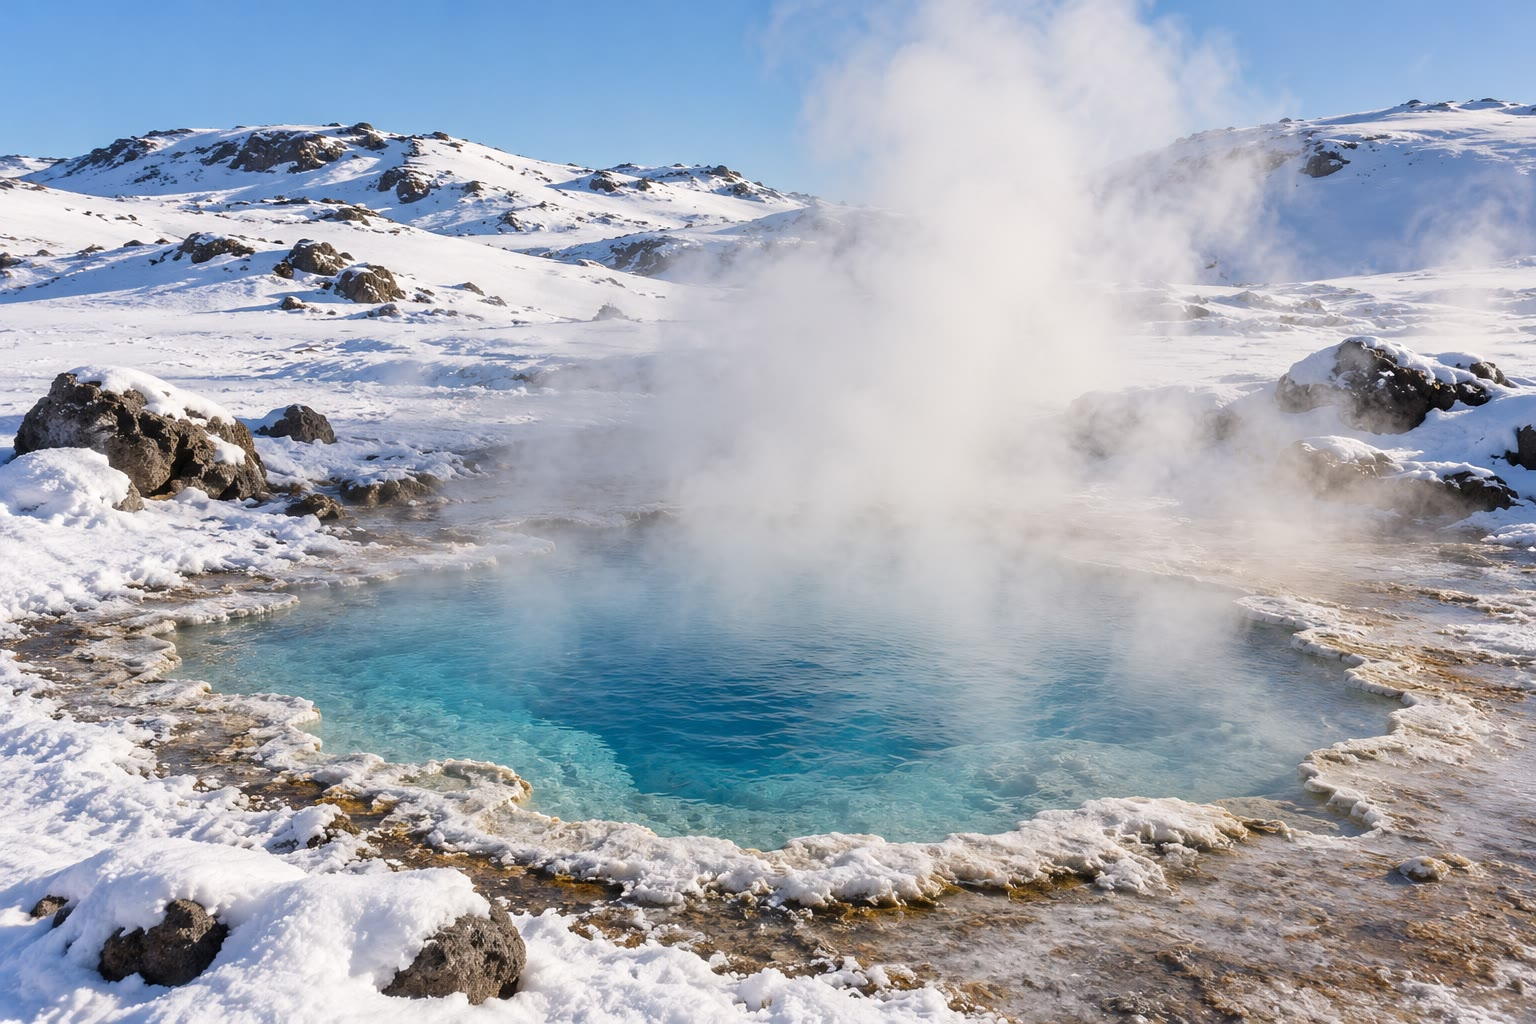
\includegraphics[width=0.6\linewidth]{images/book2/ai/g12-hot-spring-snow.jpg}

{\small Une source chaude qui fume dans un paysage enneigé~: de l'eau
réchauffée dans les profondeurs revient à la surface. Illustration générée
par IA.}
\end{omfigure}

\begin{omfigure}
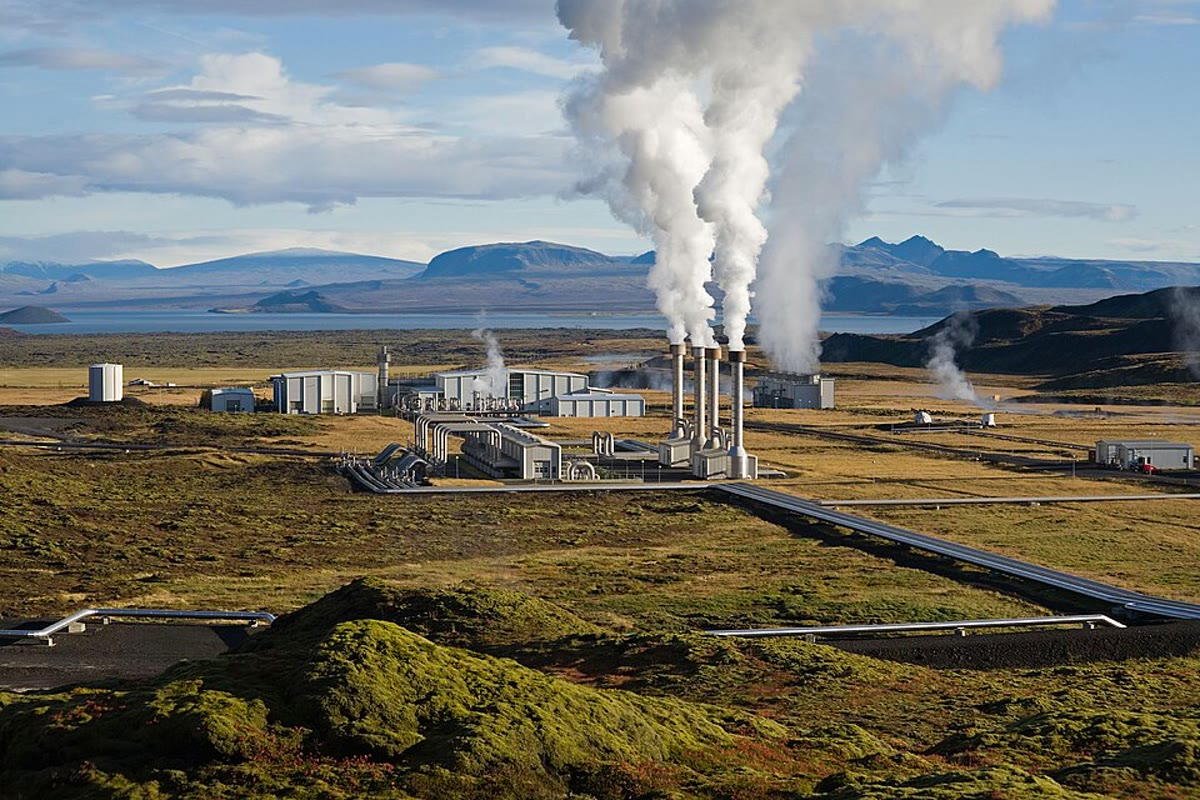
\includegraphics[width=0.66\linewidth]{images/book2/g12-nesjavellir-geothermal.jpg}

{\small La centrale géothermique de Nesjavellir, dans la région volcanique
du Hengill, en Islande~: jusqu'à \qty{120}{MW} d'électricité et jusqu'à
\qty{300}{MW} de chaleur, transportée par de l'eau chaude. Photographie
Gretar Ívarsson (domaine public).}
\end{omfigure}
% ledger: photo:g12-nesjavellir, on:nesjavellir

Un champ géothermique n'est pas inépuisable à l'échelle d'une vie humaine.
Aux Geysers, en Californie, trop de puits ont puisé la vapeur, plus vite
que le lent \omterm{def:g12:internal-heat:heat-flow}{flux géothermique} et la pluie ne pouvaient la renouveler~: la
pression de la vapeur est tombée à moins de la moitié de son maximum, et
plus de \qty{40}{\percent} de la puissance des centrales a été perdue. On
réinjecte aujourd'hui de l'eau dans le champ pour ralentir le déclin.
% ledger: cpuc:geysers

\section{Exercices}

\begin{exercise}[$\star$]\label{exo:g12:internal-heat:1}
Donner le mot~: (a) la puissance qui sort de l'intérieur à travers chaque
mètre carré de surface~; (b) la chaleur libérée par la désintégration des
atomes radioactifs dans une unité de volume de roche~; (c) la perte de la
chaleur emmagasinée depuis la formation de la Terre~; (d) le transport de
chaleur par le mouvement de la matière elle-même~; (e) la chaleur interne
de la Terre utilisée par l'homme.
\end{exercise}

\begin{exercise}[$\star$]\label{exo:g12:internal-heat:2}
Convertir~: (1) \qty{91.6}{mW/m^2} en \unit{W/m^2}~; (2) \qty{46.7}{TW} en
watts~; (3) \qty{29}{\celsius} par kilomètre en kelvins par mètre.
\end{exercise}

\begin{exercise}[$\star$]\label{exo:g12:internal-heat:3}
Nommer les quatre isotopes qui produisent presque toute la chaleur
radiogénique, et dire lesquels le détecteur KamLAND peut voir.
\end{exercise}

\begin{exercise}[$\star$]\label{exo:g12:internal-heat:4}
À l'aide de $q = 490/\sqrt{t}$, calculer le \omterm{def:g12:internal-heat:heat-flow}{flux géothermique} à travers
des fonds océaniques âgés de 1, 4, 25 et 49 millions d'années.
\end{exercise}

\begin{exercise}[$\star$]\label{exo:g12:internal-heat:5}
Pourquoi mesure-t-on le \omterm{def:g12:internal-heat:heat-flow}{flux géothermique} dans des forages plutôt qu'à la
surface même~? Pourquoi faut-il attendre après le forage avant de mesurer~?
\end{exercise}

\begin{exercise}[$\star\star$]\label{exo:g12:internal-heat:6}
Dans le forage KTB, la roche était à environ \qty{265}{\celsius} à
\qty{9.1}{km}. (1) En prenant \qty{10}{\celsius} en surface, calculer le
gradient moyen. (2) Avec une conductivité de \qty{2.72}{W/(m.K)}, quel
\omterm{def:g12:internal-heat:heat-flow}{flux géothermique} donne-t-il~? (3) Comparer à la moyenne des continents.
\end{exercise}

\begin{exercise}[$\star\star$]\label{exo:g12:internal-heat:7}
Les continents couvrent \qty{2.073e14}{m^2} avec un \omterm{def:g12:internal-heat:heat-flow}{flux géothermique} moyen
de \qty{70.9}{mW/m^2}, les océans \qty{3.028e14}{m^2} avec
\qty{105.4}{mW/m^2}. Calculer la puissance perdue par chacun, le total, et
la part perdue à travers les fonds océaniques.
\end{exercise}

\begin{exercise}[$\star\star$]\label{exo:g12:internal-heat:8}
Une couche de \omterm{def:g12:subduction-magmatism:granodiorite}{granodiorite} de \qty{8}{km} d'épaisseur a une production de
chaleur de \qty{1.88}{\micro W/m^3}. (1) Quel \omterm{def:g12:internal-heat:heat-flow}{flux géothermique}
produit-elle en surface~? (2) Quelle part cela représente-t-il de
\qty{70.9}{mW/m^2}~?
\end{exercise}

\begin{exercise}[$\star\star$]\label{exo:g12:internal-heat:9}
À quel âge les fonds océaniques perdent-ils autant de chaleur que le
continent moyen, \qty{70.9}{mW/m^2}, d'après $q = 490/\sqrt{t}$~?
\end{exercise}

\begin{exercise}[$\star\star$]\label{exo:g12:internal-heat:10}
Combien de fois plus de chaleur l'uranium~235 libérait-il il y a
1.4~milliard d'années qu'aujourd'hui~? Et le potassium~40, il y a
2.5~milliards d'années~?
\end{exercise}

\begin{exercise}[$\star\star$]\label{exo:g12:internal-heat:11}
À l'aide de $t \approx L^2/\kappa$ avec $\kappa = \qty{1e-6}{m^2/s}$,
combien de temps la chaleur met-elle à traverser par conduction (1) une
coulée de lave de \qty{10}{m} d'épaisseur~; (2) une \omterm{def:g11:lithosphere-asthenosphere:lithosphere}{lithosphère} de
\qty{100}{km} d'épaisseur~; (3) le manteau~? Exprimer chaque résultat dans
des unités adaptées.
\end{exercise}

\begin{exercise}[$\star\star\star$]\label{exo:g12:internal-heat:12}
Aujourd'hui, le thorium~232 libère environ \qty{10.4}{TW}, l'uranium~238
\qty{9.6}{TW}, le potassium~40 \qty{4.0}{TW} et l'uranium~235
\qty{0.42}{TW}. À l'aide des demi-vies de la figure, calculer la chaleur
de chacun il y a 3~milliards d'années, le total, et la part des deux
isotopes à vie courte.
\end{exercise}

\begin{exercise}[$\star\star\star$]\label{exo:g12:internal-heat:13}
La centrale de Nesjavellir peut fournir jusqu'à \qty{300}{MW} de chaleur,
transportée par environ \qty{1640}{L} d'eau chaude par seconde. Avec une
capacité thermique massique de \qty{4180}{J/(kg.K)} et une masse de
\qty{1}{kg} par litre, de combien de degrés cette eau a-t-elle été
réchauffée~? Quelle surface de continent moyen perd \qty{300}{MW} de
chaleur~?
\end{exercise}

\begin{exercise}[$\star\star\star$]\label{exo:g12:internal-heat:14}
Supposer qu'une plaque met 100 millions d'années pour aller d'une dorsale
à une fosse, et qu'une boucle de convection à travers tout le manteau en
met environ 200 millions. (1) Comparer ces durées aux 260 milliards
d'années de la conduction à travers le manteau. (2) Pourquoi la convection
peut-elle transporter la chaleur tellement plus vite, alors que le manteau
ne se déplace que de quelques centimètres par an~?
\end{exercise}

\begin{exercise}[$\star\star\star$]\label{exo:g12:internal-heat:15}
Supposer que le noyau perd environ \qty{10}{TW} de chaleur vers le manteau
à travers la \omterm{def:g11:seismic-structure:core}{limite noyau--manteau}, à \qty{2891}{km} de profondeur. (1)
Quelle part du \omterm{def:g12:internal-heat:secular-cooling}{refroidissement séculaire}, \qty{22.3}{TW}, cela
représenterait-il~? D'où vient le reste~? (2) Calculer le flux de chaleur
moyen à travers la \omterm{def:g11:seismic-structure:core}{limite noyau--manteau}, et le comparer au \omterm{def:g12:internal-heat:heat-flow}{flux
géothermique} moyen en surface, \qty{91.6}{mW/m^2}. (3) Pourquoi le noyau
chaud peut-il réchauffer la base du manteau, alors que le manteau est
solide~?
\end{exercise}

\begin{problem}[{Problème du week-end --- le bilan thermique de la Terre}]
\label{pb:g12:internal-heat:1}
% ledger: b2dd10:continents, b2dd10:half-space, kamland11:geonu, dye12:isotopes, dye12:bse, b2vila:heat-production
% values (internal_heat.py): radiogenic 24.4 TW, secular 22.3 TW, share 0.523, K40 4.0, U235 0.42, U238 9.59
Le \omterm{def:g12:internal-heat:heat-flow}{flux géothermique} de la Terre a été mesuré en plus de 38\,000 lieux. En
moyenne, les continents perdent \qty{70.9}{mW/m^2} sur
\qty{2.073e14}{m^2}, et les fonds océaniques \qty{105.4}{mW/m^2} sur
\qty{3.028e14}{m^2}.

\medskip
\noindent\textbf{Partie I --- Flux géothermique et surfaces.}
\begin{enumerate}
  \item Vérifier que les deux surfaces ont pour somme la surface d'une
        sphère de rayon \qty{6371}{km}.
  \item Quelle fraction de la surface les fonds océaniques
        représentent-ils~?
  \item Pourquoi les fonds océaniques perdent-ils plus de chaleur par mètre
        carré que les continents~?
  \item À l'aide de $q = 490/\sqrt{t}$, calculer le \omterm{def:g12:internal-heat:heat-flow}{flux géothermique} à
        travers des fonds océaniques âgés de 4 millions d'années.
  \item Un forage dans un granite (\qty{2.72}{W/(m.K)}) mesure
        \qty{26}{\celsius} par kilomètre. Son \omterm{def:g12:internal-heat:heat-flow}{flux géothermique} est-il
        supérieur ou inférieur à la moyenne continentale~?
\end{enumerate}

\medskip
\noindent\textbf{Partie II --- Le total.}
\begin{enumerate}[resume]
  \item Calculer la puissance perdue à travers les continents.
  \item Calculer la puissance perdue à travers les fonds océaniques.
  \item Les additionner~: c'est le \omterm{def:g12:internal-heat:heat-flow}{flux géothermique} total de la Terre, en
        térawatts.
  \item Quel est le \omterm{def:g12:internal-heat:heat-flow}{flux géothermique} moyen sur toute la surface~?
  \item Si \qty{10}{km} de granite (\qty{24.3}{mW/m^2}) se trouvaient sous
        tous les continents, combien de térawatts produiraient-ils~?
        Comparer à la puissance perdue à travers les continents.
\end{enumerate}

\medskip
\noindent\textbf{Partie III --- La chaleur radiogénique.}
\begin{enumerate}[resume]
  \item KamLAND compte les géoneutrinos de l'uranium~238 et du
        thorium~232~: ensemble, ils libèrent environ \qty{20.0}{TW}, avec
        \qty{3.9}{kg} de thorium dans la Terre pour chaque kilogramme
        d'uranium. Un kilogramme d'uranium libère \qty{94.4}{\micro W} par
        son uranium~238 et \qty{4.10}{\micro W} par son uranium~235~; un
        kilogramme de thorium, \qty{26.3}{\micro W}. Calculer la chaleur de
        l'uranium~238, puis celle de l'uranium~235.
  \item Le potassium~40 ajoute environ \qty{4}{TW}. Calculer la chaleur
        radiogénique totale.
  \item Quel type de roche porte l'essentiel de ces éléments, et où se
        trouve-t-il~?
  \item La chaleur radiogénique était-elle plus grande ou plus petite il y a
        3~milliards d'années~? Pourquoi~?
\end{enumerate}

\medskip
\noindent\textbf{Partie IV --- Le refroidissement séculaire.}
\begin{enumerate}[resume]
  \item Quelle puissance n'est pas fournie par la radioactivité~?
  \item D'où vient-elle~?
  \item Calculer la part du \omterm{def:g12:internal-heat:heat-flow}{flux géothermique} fournie par le
        \omterm{def:g12:internal-heat:secular-cooling}{refroidissement séculaire}.
  \item Les modèles de composition de la Terre donnent une chaleur
        radiogénique de 11 à \qty{38}{TW}. Entre quelles parts la partie
        radiogénique se situe-t-elle alors~?
  \item Qu'est-ce qui transporte l'essentiel de cette chaleur à travers le
        manteau~?
  \item Résumer~: quelle part de la perte de chaleur de la Terre la
        radioactivité fournit-elle aujourd'hui~?
\end{enumerate}
\end{problem}
